%\documentclass[draft]{article}

\documentclass[pdftex,12pt,letterpaper]{article}
\usepackage[margin=1in]{geometry}
\usepackage[pdftex]{graphicx}
\usepackage{amsmath}
\usepackage[font=footnotesize,labelfont=bf,margin=0.5in,justification=justified, singlelinecheck=on]{caption}
\usepackage{float}

% Allow superscript citations
\usepackage[superscript]{cite}

% Captions
%\usepackage[margin=0.5in,justification=justified, singlelinecheck=on]{caption}
\captionsetup[table]{singlelinecheck=on}

\newcommand{\HRule}{\rule{\linewidth}{0.5mm}}

\begin{document}

% % % % % % % % % % % % % % % % % % % % % % % % % % % % % % % % % % % % % % % %
% % % % % % % % % % % % % % % % % % % % % % % % % % % % % % % % % % % % % % % %
		% 						         Laboration														          %
% % % % % % % % % % % % % % % % % % % % % % % % % % % % % % % % % % % % % % % %
%% % % % % % % % % % % % % % % % % % % % % % % % % % % % % % % % % % % % % % % %

\begin{titlepage}
\begin{center}

% Upper part of the page. The '~' is needed because \\
% only works if a paragraph has started.

\includegraphics[width=0.5\textwidth]{./logo}~\\[1cm]

\vspace{4cm}

\textsc{\Large Biomedical Instrumentation}\\[0.5cm]

% Title
\HRule \\[0.4cm]
{ \huge \bfseries ECG Amplifier Laboration \\[0.4cm] }

\HRule \\[1.5cm]

% Author and supervisor
\noindent
\begin{minipage}{0.4\textwidth}
\begin{flushleft} \large
\emph{Authors:}\\
Courtney \textsc{Keeler} \\
Arsalan \textsc{Latif}
\end{flushleft}
\end{minipage}%
\begin{minipage}{0.4\textwidth}
\begin{flushright} \large
\emph{Professor:} \\
Dr.~Sabine \textsc{Reinfeldt} \\
\emph{Teaching Assistant:} \\
Cristina \textsc{Rigato}
\end{flushright}
\end{minipage}

\vfill

% Bottom of the page
{\large \today}

\end{center}
\end{titlepage}

\section{Introduction}

Electrocardiography (ECG) amplifiers are common  medical devices that are used to measure the electrical activity of a patient's heart. The body surface potentials that are physically measured by the device are very small in amplitude, and therefore require an amplifier that attenuates noise while amplifying the desired signal, all while protecting both the patient and the instrument. In this lab, an ECG amplifier circuit was analyzed, built, and verified on a patient in the lab.

\section{Design and Simulation}

The basic requirements for ECG circuitry are high input impedance, high gain for the desired frequency range, and high common mode rejection ratio (CMRR). These parameters are set by the circuit designer through choice of component values. The final component values are summarized in Table \ref{table:values}. Component labels correspond to those shown in Figure \ref{fig:circuit},  the overall schematic of the ECG amplifier circuit.


\begin{table}[H]
\begin{center}
    \begin{tabular}{ | l | l | }
    \hline
    Label & Value \\ \hline
    $R_{in}$ & 100 k$\Omega$ \\ \hline
    $R_1$ & 11C \\ \hline
    $R_2$ & 9C  \\ \hline
    $R_3$ & 10C  \\ \hline
    $R_4$ & 11C \\ \hline
    $R_5$ & 9C  \\ \hline
    $R_6$ & 10C  \\ \hline
    $R_7$ & 11C \\ \hline
    $R_8$ & 9C  \\ \hline
    $R_9$ & 10C  \\ \hline
    $C_1$ & 11C \\ \hline
    $C_2$ & 9C  \\ \hline
    $C_3$ & 10C  \\
    \hline
    \end{tabular}
    \caption{Final component values for the ECG amplifier circuit.}
    \label{table:values}
\end{center}
\end{table}


\begin{figure}[H]
\begin{center}
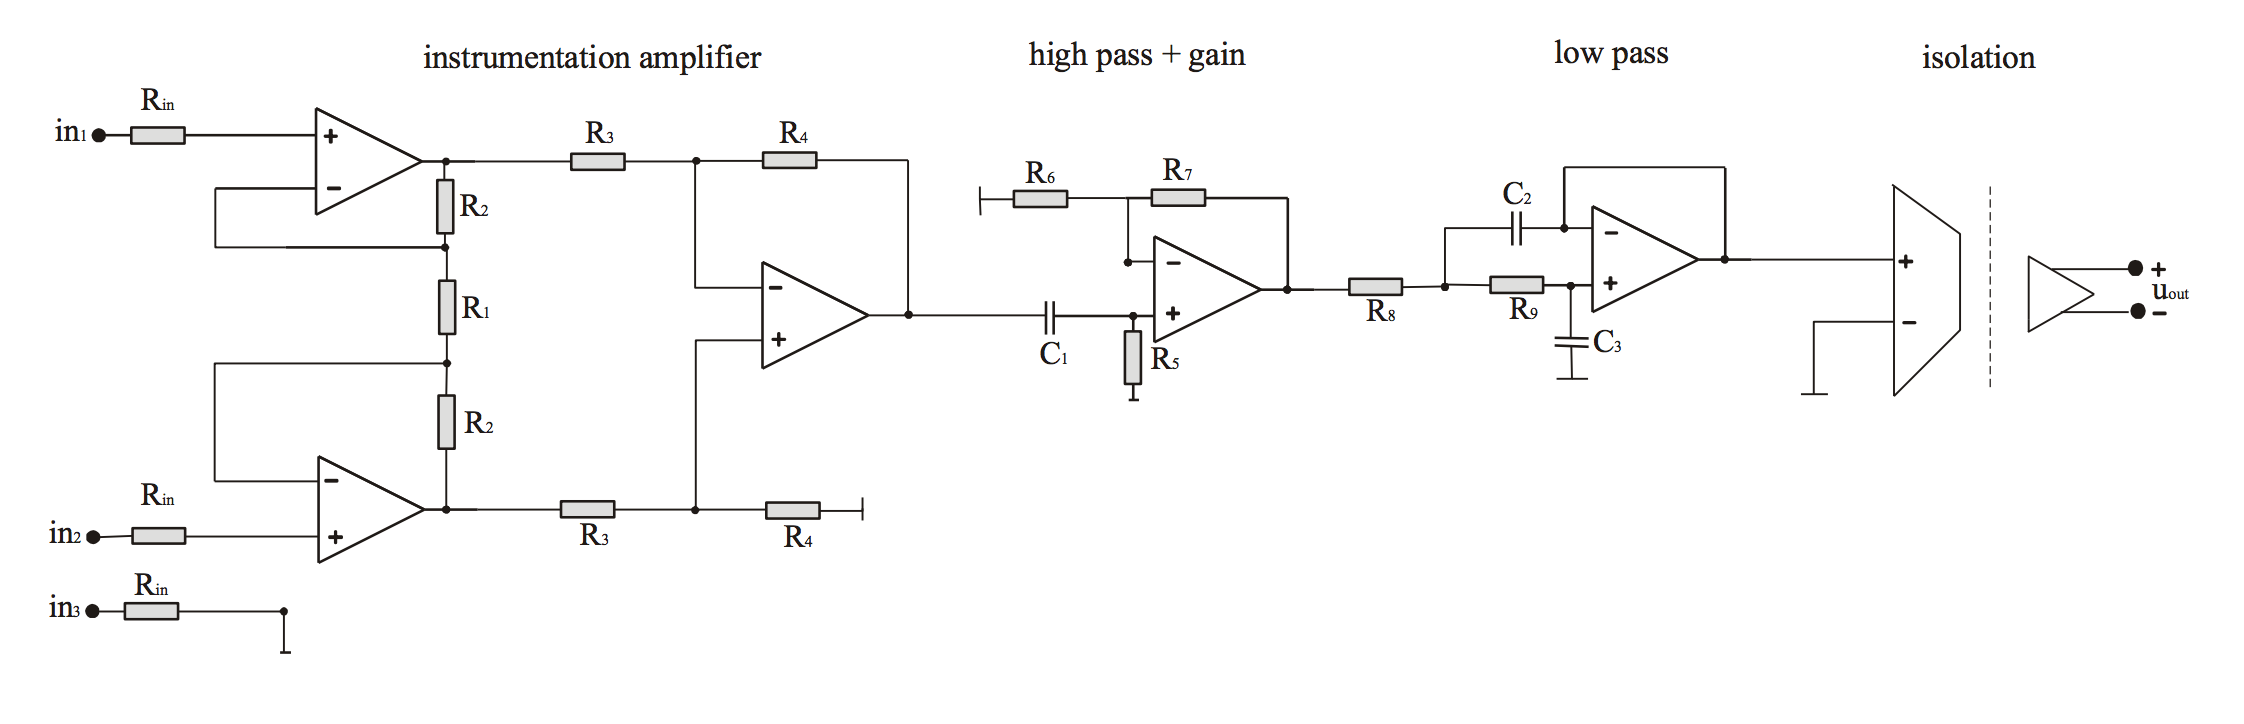
\includegraphics[scale=.35]{ECG_circuit.png}
\caption{Schematic of the circuitry used to amplify ECG signals in the laboratory.}
\label{fig:circuit}
\end{center}
\end{figure}

In total, the gain of the ECG amplifier should be 1750. However, it is bad practice to apply all of the gain at a single amplification stage, so for this reason the gain is spread between the three main stages. The first stage of the circuit, the instrumentation amplifier, was designed to have the following gain:
$$
G_1 = \frac{2R_2+R_1}{R_1}(\frac{R_4}{R_3})
$$
$$
G_1 = \frac{2(a)+b}{b}(\frac{c}{d}) = x.
$$
The second stage of the circuit, the high pass filter,  was designed to have a gain of XX. This is determined by the following equation:
$$
G_2 = R.
$$
The final stage of the circuit, the Sallen-Key low pass filter, was designed to have a gain of XX. This is set by the equation
$$
G_3 = R.
$$

In theory, the values of $R_{in}$ should be chosen such that the input impedance of the ECG amplifier circuit is sufficiently high. However, in practice if these values are too large, there is no signal seen at the output of the $R_{in}$ resistors. This is the reason for the value of 100 k$\Omega$ seen in Table \ref{table:values}.

\subsection{AC Analysis}

The final ECG circuit was simulated in two configurations in order to observe the direct mode (DM) and common mode (CM) signals. These two wiring schemes are illustrated in Figure \ref{fig:DM_CM}.

\begin{figure}[H]
\begin{center}
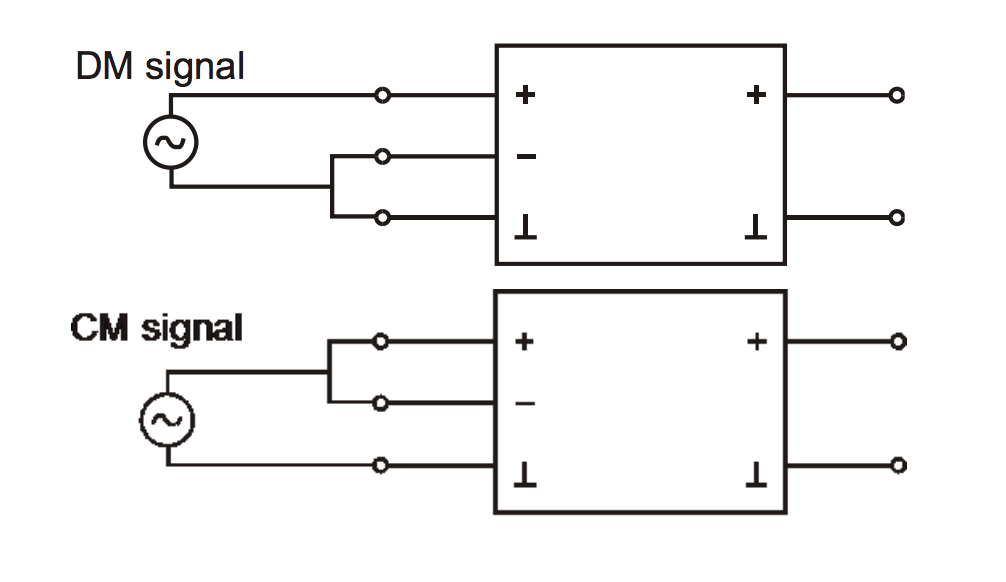
\includegraphics[scale=.5]{DM_CM.png}
\caption{Schematic of the input configurations for measuring DM and CM signals.}
\label{fig:DM_CM}
\end{center}
\end{figure}

First, the DM signals were investigated. It is desired to have a large DM signal gain; the previous section demonstrated that the gain of the ECG amplifier circuit should be XX. Figure \ref{fig:DM} shows the response of the circuit for a range of relevant frequencies. 

\begin{figure}[H]
\begin{center}
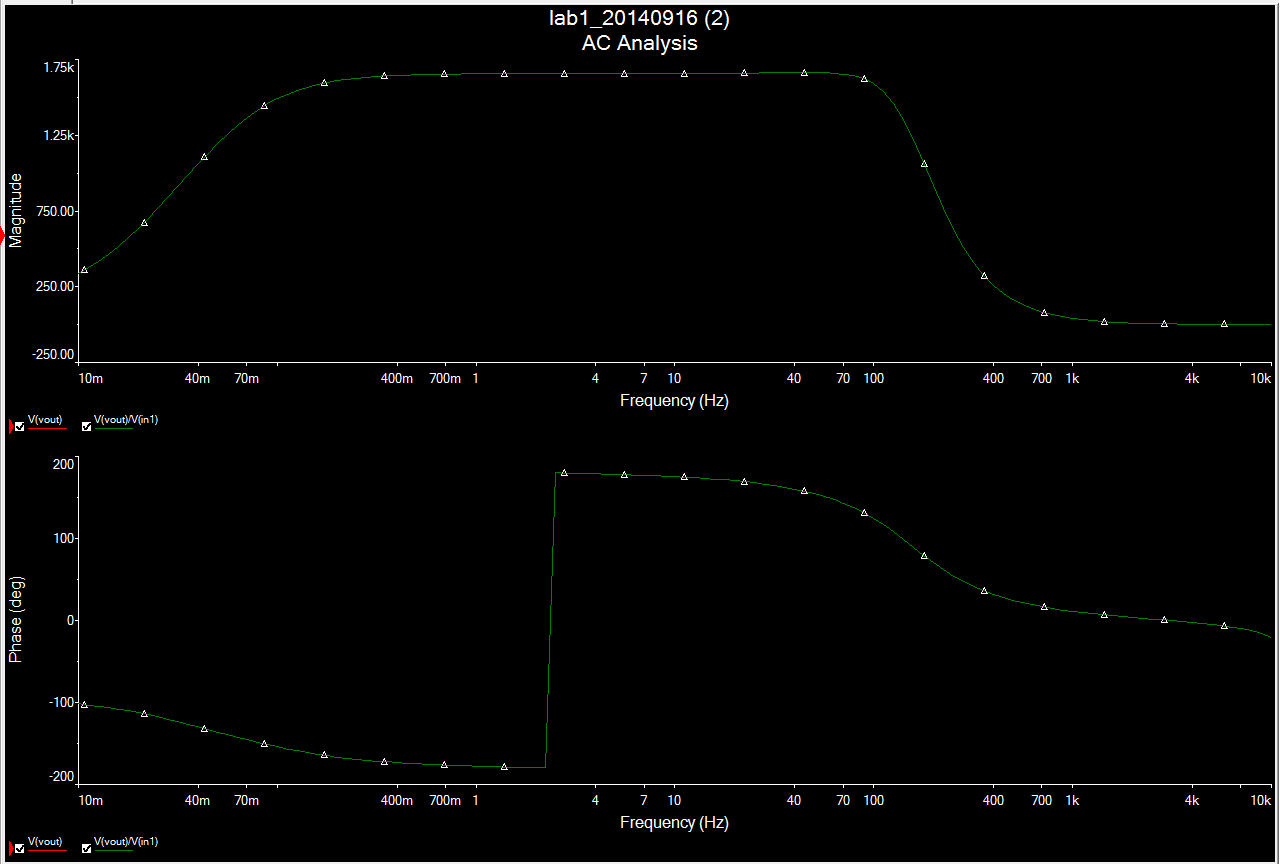
\includegraphics[scale=.35]{DM_analysis.png}
\caption{AC analysis of the simulated ECG amplifier circuit in DM measurement configuration. Notice the flat top of the magnitude spectrum. This is due to the use of a Sallen-Key filter.}
\label{fig:DM}
\end{center}
\end{figure}

It can be seen that within the range of about .4 - 100 Hz the DM signal is amplified by approximately 1750. This fits the original design requirement that the ECG amplifier have a DM gain of over 1000.

Figure \ref{fig:CM} shows the response of the circuit to CM signals over a range of simulated frequencies.
\begin{figure}[H]
\begin{center}
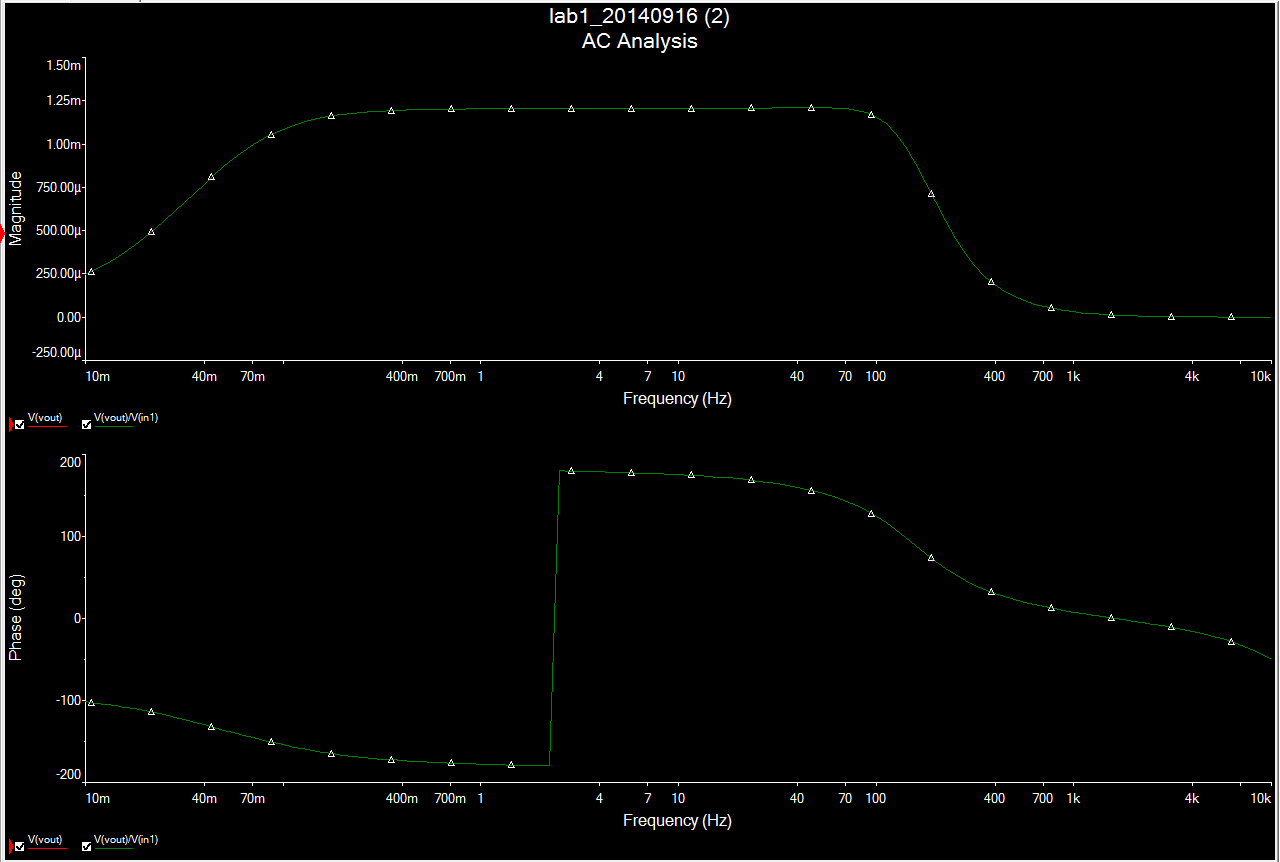
\includegraphics[scale=.35]{CM_analysis.png}
\caption{AC analysis of the simulated ECG amplifier circuit in CM measurement configuration.}
\label{fig:CM}
\end{center}
\end{figure}
In this case, a very small gain is desired. The maximum gain of these signals from the designed circuit occurs in the frequency range of about .4 - 100 Hz, and the magnitude of the gain is approximately 0.00125. In order to calculate if this value is sufficiently small, one must compute the common mode rejection ratio (CMRR). This is the ratio of the DM gain to the CM gain, as seen below:
$$
CMRR = \frac{A_{DM}}{A_{CM}} = \frac{1656.4}{.0012045} = 1375176.42
$$
This value is sufficiently large, which means that the DM and CM gains of the designed circuit are appropriate.

Figure \ref{fig:3DB} shows the frequency response of the DM circuit again, this time with the magnitude plotted in dB. This is so that the $\pm$3 dB cutoff points are easier to identify. These corner frequencies are important to know because they correspond to the range over which the above CMRR is valid. Ideally, the upper and lower corner frequencies encompass the range of frequencies present in an ECG signal so that nothing of importance is attenuated during measurement.
\begin{figure}[H]
\begin{center}
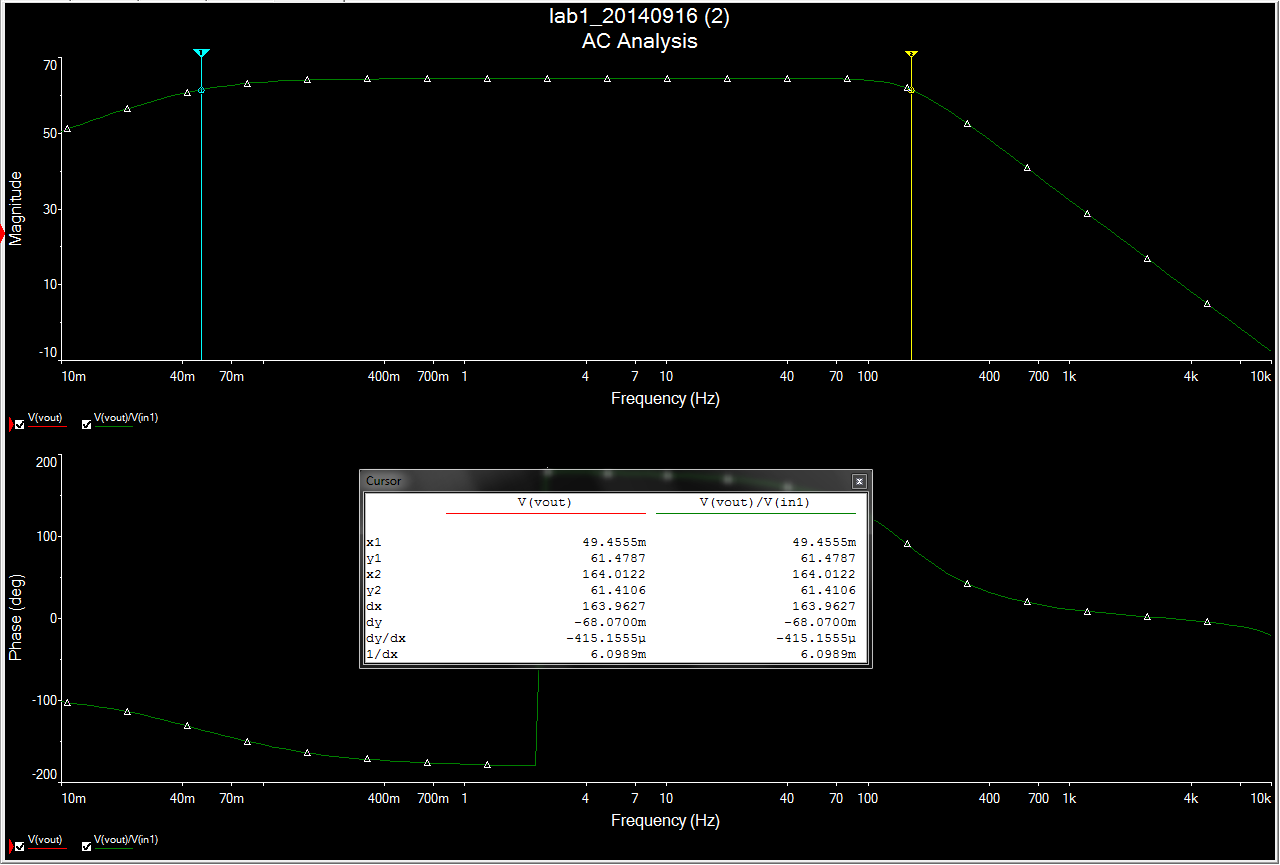
\includegraphics[scale=.35]{3db_analysis.png}
\caption{AC analysis of the simulated ECG amplifier circuit in DM measurement configuration. The y-axis is plotted in decibels in order to easily find the $\pm$3dB cutoff frequencies. Cursors 1  and 2 are placed at the lower and upper corner frequencies, respectively.}
\label{fig:3DB}
\end{center}
\end{figure}
According to Figure \ref{fig:3DB}, the lower corner frequency occurs at .049 Hz and the upper corner frequency is at 164 Hz, which is sufficient to capture the majority of the frequency components of an ECG signal.

\section{Construction and Data Acquisition}

\begin{figure}[H]
\begin{center}
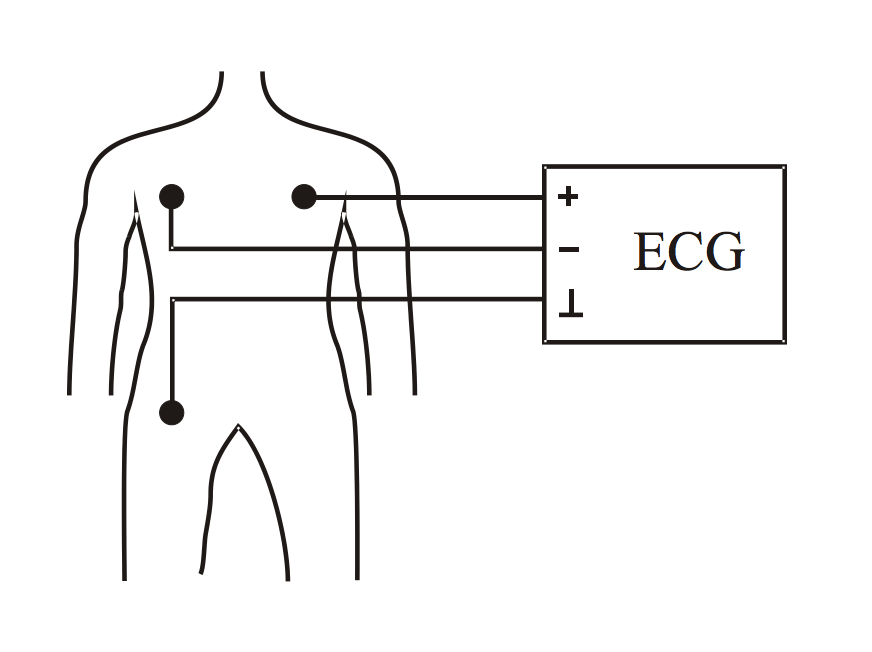
\includegraphics[scale=.5]{setup.png}
\caption{Schematic of the electrode placement for the acquisition of ECG signals in the laboratory.}
\label{fig:setup}
\end{center}
\end{figure}

\section{Results}

\begin{figure}[H]
\begin{center}
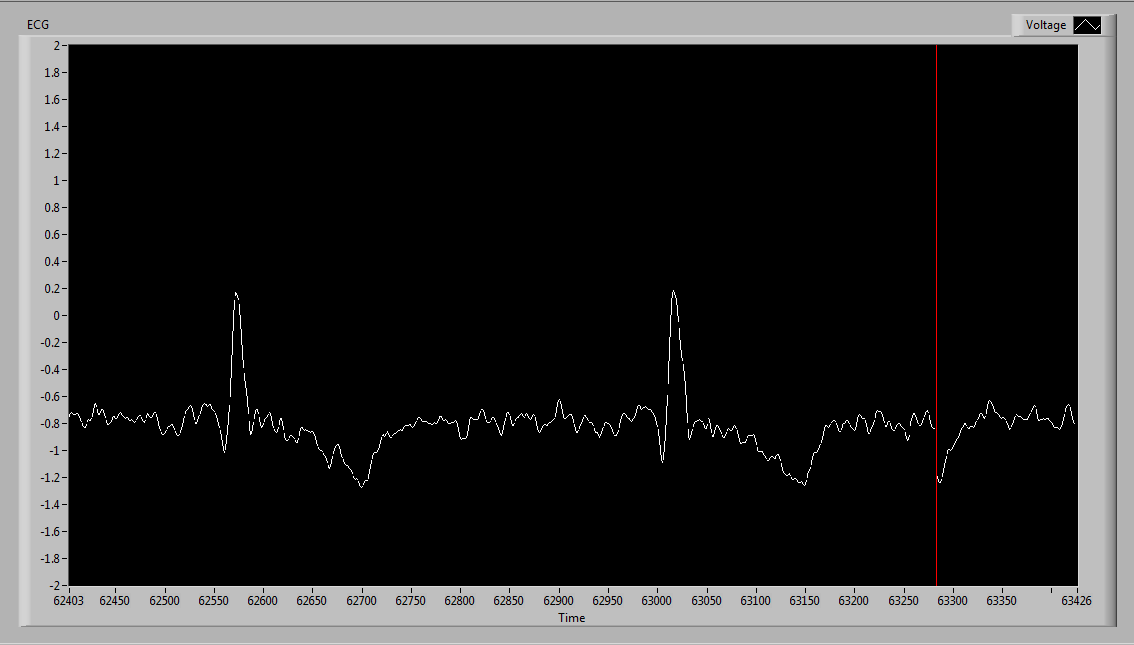
\includegraphics[scale=.4]{ECG_real.png}
\caption{Captured waveform from the ECG amplifier circuit when hooked up to electrodes placed on a patient.}
\label{fig:ECG}
\end{center}
\end{figure}

\section{Device Limitations}

Motion artifact
Using more electrodes for a better picture of heart's activity
Can't see the whole pqrst complex here, can only figure out BPM from the peaks

\begin{thebibliography}{1}

\bibitem{webster}
Webster, John G. Medical Instrumentation Application and Design, 4th Edition. John Wiley \& Sons, 092008. VitalBook file.

\end{thebibliography}

\end{document}